
\begin{table}[H]
\begin{adjustbox}{width=\textwidth}
\begin{tabular}{lllllll}
\textbf{Rows} & \textbf{1} & \textbf{10} & \textbf{100} & \textbf{1000} & \textbf{10000} & \textbf{100000} \\
\textbf{Initial load} & 96.7 $\pm$ 2.38 & 98.67 $\pm$ 5.52 & 103.77 $\pm$ 2.72 & 140.63 $\pm$ 3.67 & 409.73 $\pm$ 5.09 & 2888.3 $\pm$ 0\\
\textbf{Subsequent load} & 48.58 $\pm$ 1.12 & 48.95 $\pm$ 1.41 & 50.51 $\pm$ 3.4 & 49.8 $\pm$ 2.69 & 49.87 $\pm$ 1.32 & 39.09 $\pm$ 0.74\\
\textbf{Select 1 rows} & 0.47 $\pm$ 0.25 & 0.48 $\pm$ 0.25 & 0.48 $\pm$ 0.08 & 0.48 $\pm$ 0.2 & 0.46 $\pm$ 0.19 & 0.48 $\pm$ 0.37\\
\textbf{Select 10 rows} & 0.46 $\pm$ 0.09 & 0.55 $\pm$ 0.12 & 0.55 $\pm$ 0.15 & 0.56 $\pm$ 0.13 & 0.57 $\pm$ 0.18 & 0.55 $\pm$ 0.11\\
\textbf{Select 100 rows} & 0.46 $\pm$ 0.14 & 0.55 $\pm$ 0.12 & 1.49 $\pm$ 0.27 & 1.41 $\pm$ 0.23 & 1.41 $\pm$ 0.22 & 1.54 $\pm$ 2.84\\
\textbf{Select 10 joined} & 0.5 $\pm$ 0.09 & 0.61 $\pm$ 0.13 & 0.64 $\pm$ 0.24 & 0.64 $\pm$ 0.15 & 0.64 $\pm$ 0.12 & 0.64 $\pm$ 0.13\\
\textbf{Update reservation} & 10 $\pm$ 1.18 & 10.37 $\pm$ 1.03 & 11.06 $\pm$ 0.84 & 11.17 $\pm$ 1.12 & 11.28 $\pm$ 1.04 & 11.49 $\pm$ 1.62\\
\textbf{Create reservation} & 12.15 $\pm$ 1.38 & 11.6 $\pm$ 2.19 & 10.38 $\pm$ 2.28 & 10.46 $\pm$ 2.09 & 11.18 $\pm$ 2.24 & 18.87 $\pm$ 2.41\\
\textbf{Delete reservation} & 13.05 $\pm$ 0.75 & 13.16 $\pm$ 0.81 & 13.37 $\pm$ 1.16 & 13.04 $\pm$ 0.73 & 13.19 $\pm$ 1.31 & 12.64 $\pm$ 0.58
\end{tabular}
\end{adjustbox}
\caption{Duration in milliseconds of client-side operations for databases with different number of rows.}
\label{tab:client-experiment }
\end{table}
    
\begin{figure}[H]
    \centering

\begin{subfigure}[b]{0.48\textwidth}
    \centering
    
\resizebox{\textwidth}{!}{
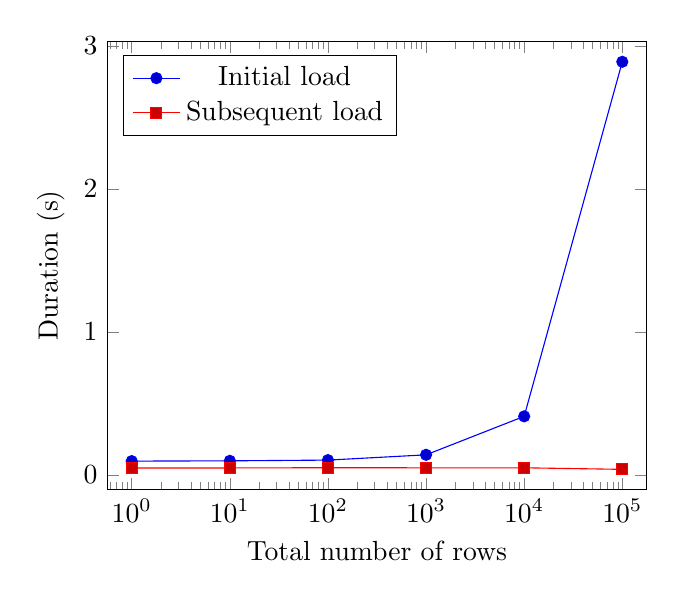
\begin{tikzpicture}
\begin{axis}[
    scaled x ticks=false,
    xticklabel style={
        /pgf/number format/fixed,
    },
    enlargelimits=0.05,
    xmode=log,
    legend pos=north west,
	ylabel=Duration (s),
    xlabel=Total number of rows,
]
\addplot coordinates {
(1,0.09669999999976293)
(10,0.09867272727242248)
(100,0.10377000000011176)
(1000,0.14062500000023284)
(10000,0.409733333333085)
(100000,2.8882999999988823)
};
\addplot coordinates {
(1,0.0485809523810056)
(10,0.048952380952203556)
(100,0.050514999999664724)
(1000,0.049804761905045736)
(10000,0.04986666666663119)
(100000,0.03909230769225038)
};
\legend{Initial load,Subsequent load}
\end{axis}
\end{tikzpicture}

}

    \caption{Duration in seconds of setting up and loading the data for a new and existing Relic instance by total number of rows.}
    \label{fig:client-load-times}
\end{subfigure}
\hfill
\begin{subfigure}[b]{0.48\textwidth}
    \centering
    
\resizebox{\textwidth}{!}{
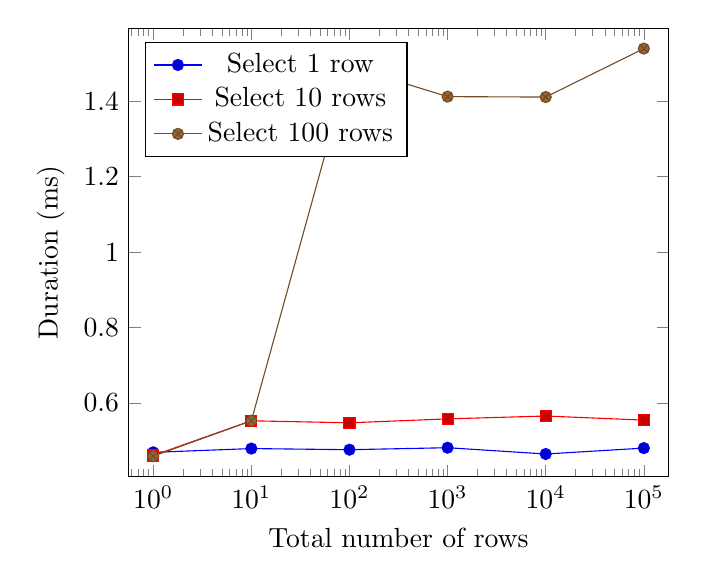
\begin{tikzpicture}
\begin{axis}[
    scaled x ticks=false,
    xticklabel style={
        /pgf/number format/fixed,
    },
    enlargelimits=0.05,
    xmode=log,
    legend pos=north west,
	ylabel=Duration (ms),
    xlabel=Total number of rows,
]
\addplot coordinates {
(1,0.4687441424575775)
(10,0.47874581139461597)
(100,0.47573739295908657)
(1000,0.4810004810031688)
(10000,0.4643454038959166)
(100000,0.4799904030713748)
};
\addplot coordinates {
(1,0.46037735849073746)
(10,0.5524572059656131)
(100,0.5470749043190964)
(1000,0.55752508360851)
(10000,0.565084745762291)
(100000,0.5542382271480527)
};
\addplot coordinates {
(1,0.45859697386400383)
(10,0.5524861878453039)
(100,1.4928358208944104)
(1000,1.4125706214684004)
(10000,1.4114245416094748)
(100000,1.5400000000028655)
};
\legend{Select 1 row,Select 10 rows,Select 100 rows}
\end{axis}
\end{tikzpicture}

}

    \caption{Duration in milliseconds of selecting 1, 10 and 100 rows by total number of rows in the database.}
    \label{fig:client-select-n}
\end{subfigure}
\\
\begin{subfigure}[b]{0.48\textwidth}
    \centering
    
\resizebox{\textwidth}{!}{
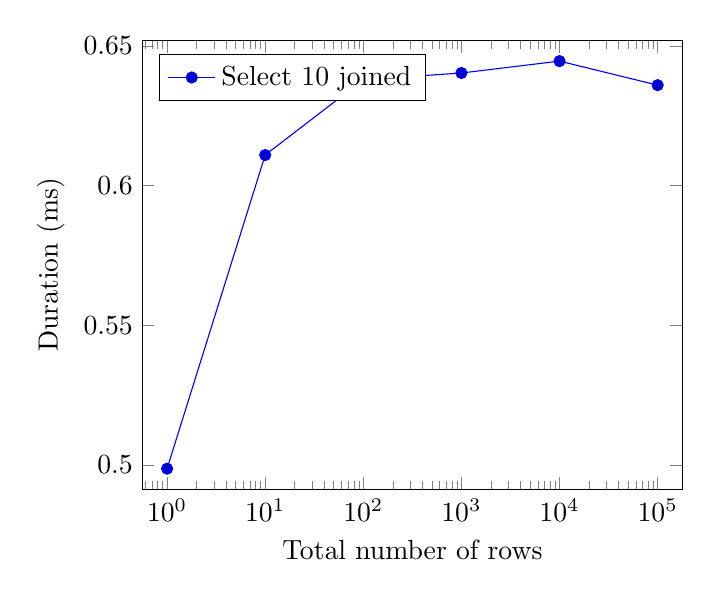
\begin{tikzpicture}
\begin{axis}[
    scaled x ticks=false,
    xticklabel style={
        /pgf/number format/fixed,
    },
    enlargelimits=0.05,
    xmode=log,
    legend pos=north west,
	ylabel=Duration (ms),
    xlabel=Total number of rows,
]
\addplot coordinates {
(1,0.49870388833610924)
(10,0.6109279609263689)
(100,0.6378826530607493)
(1000,0.6402688860456803)
(10000,0.6445231958743685)
(100000,0.6359186268270073)
};
\legend{Select 10 joined}
\end{axis}
\end{tikzpicture}

}

    \caption{Duration in milliseconds of selecting 10 rows using a join by total number of rows in the database.}
    \label{fig:client-select-advanced}
\end{subfigure}
\hfill
\begin{subfigure}[b]{0.48\textwidth}
    \centering
    
\resizebox{\textwidth}{!}{
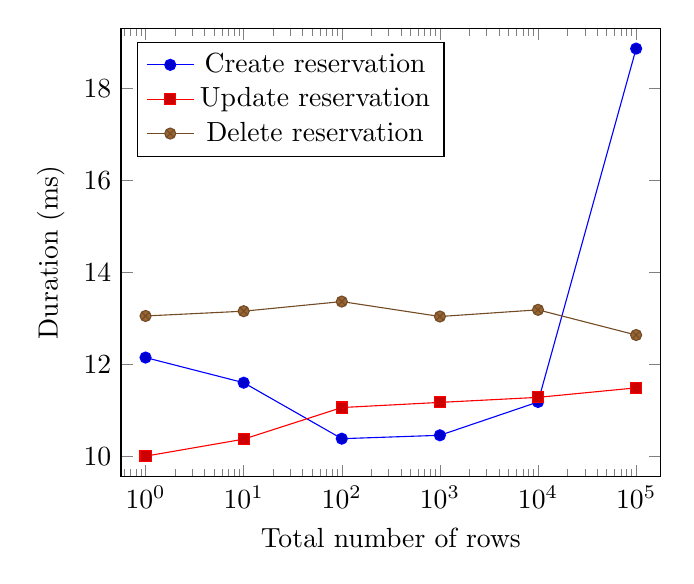
\begin{tikzpicture}
\begin{axis}[
    scaled x ticks=false,
    xticklabel style={
        /pgf/number format/fixed,
    },
    enlargelimits=0.05,
    xmode=log,
    legend pos=north west,
	ylabel=Duration (ms),
    xlabel=Total number of rows,
]
\addplot coordinates {
(1,12.148192771138197)
(10,11.601149425146053)
(100,10.382474226896296)
(1000,10.45624999993015)
(10000,11.181111111098694)
(100000,18.87222222218083)
};
\addplot coordinates {
(1,10.001980198012426)
(10,10.37216494846897)
(100,11.06043956043956)
(1000,11.172222222201526)
(10000,11.282022471905927)
(100000,11.488636363636363)
};
\addplot coordinates {
(1,13.053246753217724)
(10,13.15714285711383)
(100,13.366666666517656)
(1000,13.041558441669716)
(10000,13.186842105351388)
(100000,12.638749999948777)
};
\legend{Create reservation,Update reservation,Delete reservation}
\end{axis}
\end{tikzpicture}

}

    \caption{Duration in milliseconds to completion of mutations by total number of rows in the database.}
    \label{fig:client-mutations}
\end{subfigure}
    
    \caption{Latency of various client-side Relic operations for the meeting room scheduler}
    \label{fig:client-experiment}
\end{figure}
